\chapter{Memory}
\label{chp:memory}
\index{Memory}

\section{Introduction} 
\index{Memory!Structure}

\newcommand{\memoryLayout}[1]
{

	\begin{figure}[htp!] \small
		\centering
		\begin{tabular}{|c|c|c|}
			\toprule
			\textbf{Page no} & \textbf{Contents} & \textbf{Word addr} \\
			\toprule 
			0   & \hyperref[lbl:romcode]{ROM code} 		& 0 -- 255 \\ \hline 
			1   & \hyperref[lbl:oscode]{OS Startup code} 	& 256 -- 511  \\ \hline 
			\multirow{5}{*}{2} 
				& \hyperref[lbl:pgtbl]{Static Page Tables}   & 512 -- 559 \\ \cline{2-3} 
				& \hyperref[lbl:memlst]{Memory Free List}  & 560 -- 623  \\ \cline{2-3}
				& \hyperref[lbl:gft]{Global File Table}  & 624 -- 719 \\ \cline{2-3}
				& \hyperref[lbl:rdylst]{Ready List} & 720 -- 731 \\ \cline{2-3}
				& Unallocated & 732 -- 767 \\ \hline 
			\multirow{2}{*}{3}
				& \hyperref[lbl:proctbl]{Process Table} & 768 -- 959 \\ \cline{2-3}
				& Unallocated & 960 -- 1023 \\ \hline 
			4 & \multirow{2}{*}
				{\hyperref[lbl:fat]{File Allocation Table}} & \multirow{2}{*}{1024 -- 1535} \\ \cline{1-1} 
			5 & 				 &  \\ \hline 
			6 & \multirow{2}{*}
				{\hyperref[lbl:disklst]{Disk Free List}} & \multirow{2}{*}{1536 -- 2047}\\ \cline{1-1} 
			7 & 				& \\ \hline 
			8 & \multirow{3}{*}
				{\hyperref[lbl:INITprocess]{INIT process}} & \multirow{3}{*}{2048 -- 2815} \\ \cline{1-1} 
			9 & 				 &  \\ \cline{1-1} 
			10 & 				 &  \\ \hline 
			\multirow{3}{*}{11 -- 55}
				&  \vdots & \\   
				&  User Programs & 2816 -- 14335 \\  
				& \vdots & \\ \hline 
			56 & \hyperref[lbl:int]{INT 0} & 14336 -- 14591 \\ \hline 
			57 & \hyperref[lbl:int]{INT 1} & 14592 -- 14848 \\ \hline 
			\vdots & \vdots & \vdots \\ \hline 
			63 & \hyperref[lbl:int]{INT 7} & 16128 -- 16383 \\  
			\bottomrule
		\end{tabular}
		\caption{Outline of the main memory}
		\label{#1}
		\index{Memory!Structure}
	\end{figure}

}

\memoryLayout{fig:main memory}

\begin{itemize}
	\item The basic unit of memory in the \ESIM architecture is a word. \index{Memory!Word}
	\item The machine memory can be thought of as a linear sequence of words.
	\item A collection of 256 contiguous words is known as a \emph{page}. \index{Memory!Page}
	\item The total size of the memory is 64 pages or 16384 ($256 \times 64$) words.
	\item Each word in the memory is identified by the \emph{word address} in the range 0 to $16383(256 \times 64 - 1)$. Similarly, each page in the memory is identified by the \emph{page number} \index{Memory!Page number} in the range 0 to 63.
\end{itemize}

\begin{example}
	The $256^{th}$ word of the memory has a word address 255 and belongs to page 0. In general, the $n^{th}$ word has the word address $(n-1)$, where  $1 \le n \le 16384$ and belongs to the page $\lfloor \frac{n-1}{256} \rfloor$. Refer figure~\ref{fig:mem_struct}. 
\end{example}

\begin{figure}[htp!] \small
	\centering
	\begin{tabular}{c|c|c|} 
		\multicolumn{3}{c}{} \\
		\textbf{Word address} &  & \textbf{Page no.} \\ \cline{2-3}
		0 & $1^{st}$ word & \multirow{4}{*}{$0$} \\ \cline{2-2}
		1 & $2^{nd}$ word &  \\ \cline{2-2}
		\vdots & \vdots & \\ \cline{2-2}
		255 & $256^{th}$ word &  \\ \cline{2-3}
	
		\vdots & \vdots & \multirow{2}{*}{$\lfloor \frac{i}{256} \rfloor $} \\ \cline{2-2}
		$i$ & $(i+1)^{th} $ word &  \\ \cline{2-2}
		\vdots &\vdots &  \\ \cline{2-3}
	
		\vdots & \vdots & \multirow{2}{*}{$63$} \\ \cline{2-2}
		\vdots &\vdots &  \\ \cline{2-2}
		$256 \times 64 - 1$ & $(256 \times 64)^{th} $ word &  \\ \cline{2-3}
	\end{tabular}
	\caption{Illustration of memory addressing}
	\label{fig:mem_struct}
\end{figure}

\section{Page Table}
\index{Page Table}

Before explaining the page table, we explain two well known terms:
\begin{itemize}
	\item \textbf{Logical address :} It is the CPU generated address of the data. 
	\item \textbf{Physical address :} It is the exact location of the data in the main memory.
\end{itemize}

\begin{figure}[h!]
	\centering
	\includegraphics[scale=0.55]{pics/paging}
	\caption{Paging model of the \ESIM architecture}
	\label{fig:paging}
	\index{Page Table!Paging Model}
\end{figure}

Refer ``Memory management strategies" in the book \cite{galvin} to know more about paging. 

The page table contains information relating to the actual location in the memory, i.e., the physical address, of the data specified by the logical address. Each entry of a page table contains the page number in the memory where the data specified by the logical address resides. Refer figure~\ref{fig:paging}.


\section{Address Translation} 
\index{Address Translation}
It is the process of obtaining the physical address from the logical address. It is done by the machine in the following way. Refer book~\cite{Bach} for more details.

\begin{enumerate}
	\item The logical address generated by the CPU is divided by the page size (256) to get the \emph{logical page number}.
	\item The remainder got after performing the above division gives the \emph{offset} within that page.
	\item The \emph{logical page number} is then used to index the page table to get the corresponding \emph{physical page number} in the memory.
	\item The \emph{offset} got in step 2 is then used to refer to the word in the physical page containing the data.\\
\end{enumerate}

\begin{figure}[h!]
	\centering
	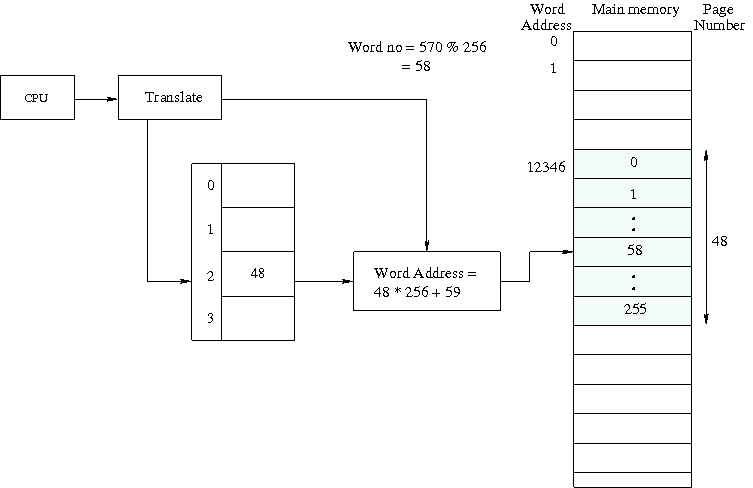
\includegraphics[scale=0.55]{pics/paging_example}
	\caption{Diagram illustrating address translation}
	\label{fig:paging_example}
\end{figure}

\begin{example}
	Consider the scenario in figure~\ref{fig:paging_example}. Here the logical address generated is 570, so the page number is $ \lfloor 570/265 \rfloor = 2$ and word address is $570\mbox{ mod }256 = 58$. The looked up value from the page table is $48$. Thus the resultant physical address is $48 \times 256+58$.
\end{example}
	
\section{Memory Free List}
\label{lbl:memlst}
\index{Memory!Free list}

\begin{itemize}
	\item The free list of the memory consists of 64 entries. Each entry is of size one word.
	\item The total size of the free list is thus 64 words (64 (= no. of entries) $\times$ 1 (= size of one entry) = 64 words).
	\item It is present in the second 64 words of page 2 of the memory. Refer figure~\ref{fig:main memory}.
	\item Each entry of the free list contains a value of either 0 or 1 indicating whether the corresponding page in the memory is free or not respectively.
\end{itemize}

\begin{example} 
	Figure~\ref{fig:mem_free_list} indicates that pages 0, 1 and 63 of the memory are not free while pages 2 and 48 are free.
\end{example}

\begin{figure}[htp!] \small
	\centering
	\begin{tabular}{c|c|}
%		\multicolumn{2}{c}{} \\ 
		\textbf{Pg no.} & \textbf{Contents} \\ \cline{2-2}
		$0$ & $1$ \\ \cline{2-2}
		$1$ & $1$ \\ \cline{2-2}
		$2$ & $0$ \\ \cline{2-2}
		\vdots & \vdots \\ \cline{2-2}
		$48$ & $0$ \\ \cline{2-2}
		$\vdots$ & \vdots \\ \cline{2-2}
		$63$ & $1$ \\ \cline{2-2}
	\end{tabular}
	\caption{A sample free list of the memory}
	\label{fig:mem_free_list}
\end{figure}

The entire structure of memory is outlined in figure~\ref{fig:main memory}.
